%% \section[Quick Recall of Convexity]{Quick Recall of Convexity}

%% \begin{frame}
%%   \frametitle{Table of Contents}
%%   \tableofcontents[currentsection]
%% \end{frame}

\begin{frame}{Quick Recall of Convexity}
  \begin{itemize}
  \item Strong Convexity
  %% \item Sub-differential (sub-gradient)
  \item Convex Conjugate
  \item Dual Norm
  \item Strong Smoothness
  \end{itemize}
\end{frame}

\begin{frame}{Convexity}
  Recall a function is convex if,
  \begin{align*} 
    \underbrace{\f(\x) + \dotprod{\grad \f(\x)}{\y-\x}}_{\text{the value at $\y$ of the tangent at $\x$}} \le \f(\y) \\
    \text{Rearranging, } \f(\x)-\f(\y) \le \dotprod{\grad \f(\x)} {\x-\y} \\
  \end{align*}
  \begin{figure}
    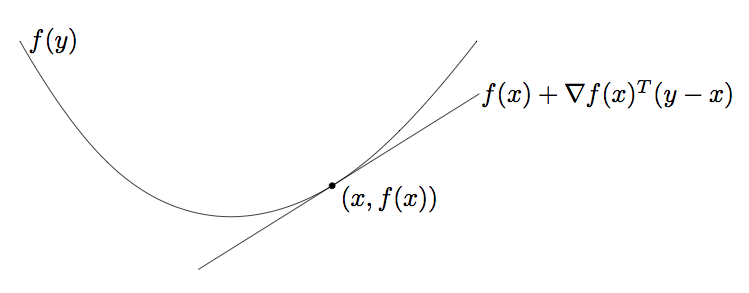
\includegraphics[scale=0.27]{images/convexity.png}
    \caption{From \cite{BV2004}}
  \end{figure}
\end{frame}

\begin{frame}{Strong Convexity}
  A function $\f$ is said to be $\beta$-strongly convex (wrt norm $\|\|$) if,
  \begin{align*}
   & \f(\y) \ge \underbrace{\f(\x) + \dotprod{\grad \f(\x)}{\y-\x}}_{\text{the value at $\y$ of the tangent at $\x$}} + \frac{\beta}{2} \|\y-\x\|^2\\
   %% & \text{Substituting x+y for y,} \\
   %% & \f(\x+\y) \ge \f(\x) + \dotprod{\grad \f(\x)}{\y} +\frac{\beta}{2} \|\y\|^2
  \end{align*}
  %% Equivalently,
  %% \begin{align*}
  %%   \f(\alpha \x +(1-\alpha)\y) \le \alpha \f(\x) + (1-\alpha)\f(\y) - \alpha(1-\alpha)\frac{\beta}{2} \|\y-\x\|^2
  %% \end{align*}
\end{frame}

\begin{frame}{Strong Convexity}
  \begin{figure}
    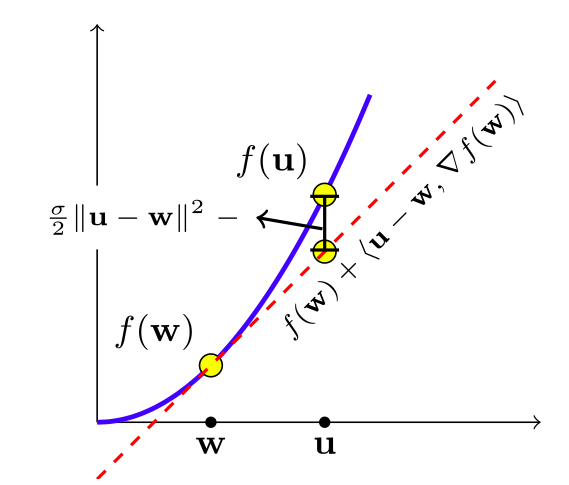
\includegraphics[scale=0.27]{images/str_convex.png}
    \caption{From \cite{ShSh2012}. A $\sigma$ strongly convex function.}
  \end{figure}
\end{frame}


\begin{frame}{Convex Conjugate}
  (Also called Fenchel Conjugate)\\
  {\bf Idea:} There is a unique tangent to a convex function of a given slope $\y$. Therefore, a convex function can be uniquely represented by $(x,f(x))$ or alternatively by (slope,intercept with y-axis).
  \begin{definition}
    The convex conjugate of a function $\f$, denote by $\opt{\f}$ is defined as,
    \begin{align*}
      \opt{\f}(\y) = \max_{\x} \dotprod{\x}{\y} - \f(\x)
    \end{align*}
    $\opt{\f}(\y)$ answers the question:``what is the intercept of the tangent to $\f$ which has slope $\y$?''
  \end{definition}
  Note that $\opt{\f}(\y)$ will be unique and convex.
\end{frame}


\begin{frame}{Convex Conjugate}
  \begin{figure}
    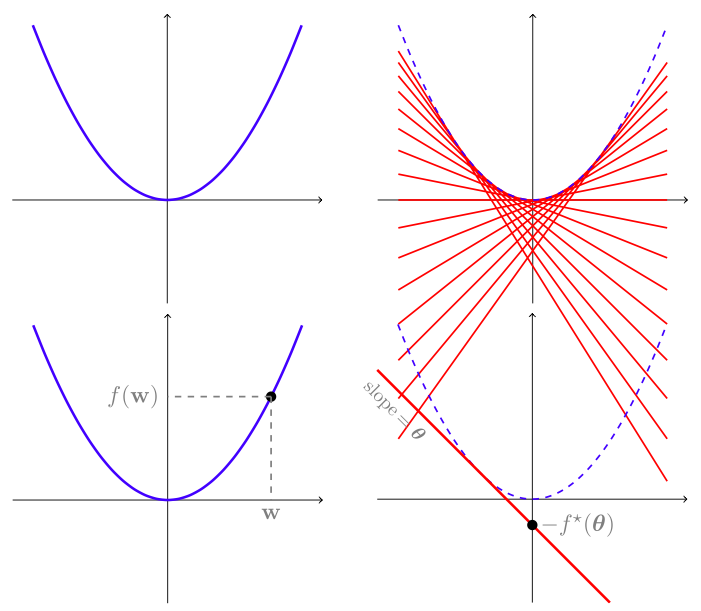
\includegraphics[scale=0.27]{images/fenchel.png}
    \caption{From \cite{ShSh2012}}
  \end{figure}
\end{frame}

\begin{frame}{Important Properties of Conjugates}
  \begin{itemize} 
  \item Derivatives of Conjugates
    \begin{align*}
    \nabla \opt{\f}(\y) = \argmax_{\x}\dotprod{\x}{\y} - \f(\x)
  \end{align*}  
  \item From the definition of Fenchel conjugate, we have the following inequality,
    \begin{align*}
      \f(\x) + \opt{\f}(\y) \ge \dotprod{\x}{\y} \tag{Fenchel Young Inequality}
    \end{align*}
  \end{itemize}

\end{frame}

\begin{frame}{Dual Norm}
  The dual norm of the norm $\| \cdot \|$ is given by
  \begin{align*}
    \|y\|_{*} = \sup\{\dotprod{x}{y} : \|x\| \le 1\}
  \end{align*}
      {\bf Important Property:} Fenchel conjugate of $\frac{\|\x\|^2}{2}$ is $\frac{\|\x\|_{*}^2}{2}$.
      \begin{center}
        \begin{tabular}{ll}
          Norm & Dual Norm\\
          \hline
          $l_2$ & $l_2$\\
          $l_1$ & $l_{\infty}$\\
          $l_p$ & $l_q$ where $\frac{1}{p}+\frac{1}{q}=1$\\
        \end{tabular}
      \end{center}
\end{frame}

\begin{frame}{Strong Smoothness}
  A function is said to be $\beta$-strongly smooth (wrt norm $\| \cdot \|$) if,
  \begin{align*}
    \f(\x+\y) \le \f(\x) + \dotprod{\grad \f(\x)}{\y} +\frac{\beta}{2} \|\y\|^2
  \end{align*}
  Note the difference in direction of inequality from strong convexity.
\end{frame}

\begin{frame}{Strong Convexity/Strong Smoothness Duality}
  \begin{theorem}[6]
    Assume $\f$ is a closed and convex function. Then
    \begin{align*}
      \f \text{ is } \beta\text{-strongly convex wrt }  \| \cdot \| \iff \opt{\f} \text{ is } \frac{1}{\beta}\text{-smooth wrt }  \| \cdot \|_{*}
    \end{align*}
  \end{theorem}
\end{frame}

\begin{frame}{A Useful Lemma}
  \begin{lemma}
    If $\f$ is $\beta$ strong convex wrt $\|\cdot\|$ and $\opt{\f}(0)=0$, then for any sequence $v_1,v_2,...,v_n$ and any $u$, we have,
    \begin{align*}
      \sum_{i=1}^n \dotprod{v_i}{u} - f(u) \le \opt{\f}(v_{1:n}) \le \sum_{i=1}^n \dotprod{\grad \opt{\f}(v_{1:i-1})}{v_i} +\frac{1}{2\beta} \sum_{i=1}^n \|v_i\|_{*}^2
    \end{align*}
    where $v_{1:n}=\sum_1^n v_i$.
  \end{lemma}
\end{frame}

\begin{frame}
    \begin{align*}
      & \sum_{i=1}^n \dotprod{v_i}{u} - f(u) \le \opt{\f}(v_{1:n}) \tag{Fenchel-Young} \\
      & \opt{\f}(v_{1:n}) \le \sum_{i=1}^n \dotprod{\grad \opt{\f}(v_{1:i-1})}{v_i} +\frac{1}{2\beta} \sum_{i=1}^n \|v_i\|_{*}^2
    \end{align*}
    Induction on the definition of smoothness.
    \begin{align*}
      \opt{\f}(v_{1:n-1}+v_n) \le \opt{\f}(v_{1:n-1}) + \dotprod{\grad \opt{\f}(v_{1:n-1})}{v_n} +\frac{\beta}{2} \|v_n\|_{*}^2
    \end{align*}

\end{frame}
%% \section[]{Follow the Regularized Leader}


\begin{frame}{Generalized Regret Bound}
  \begin{align*}
    Regret(\w_1,\w_2,\cdots,\w_T,u) = \sum_{t=1}^T l_t(w_t) - \min_{u \in S} \sum_{t=1}^T l_t(u)
  \end{align*}
\end{frame}

\begin{frame}{Follow the Regularized Leader (FoReL)}
  \begin{align*}
    w_{t+1} = \argmin_w \sum_{s=1}^t l_s(w) + f(w) \tag{Main Idea}
  \end{align*}
  \begin{figure}
  \begin{algorithmic}[1]
    \Let{$\w_1$}{$\grad \opt{f}(0)$} 
    \For{$t=1$ ... $T$}
    \State Play $\w_t \in S$
    \State Receive $l_t$ and pick $v_t \in \partial l_t(w_t)$
    \State Update,
    \Let{$w_{t+1}$}{$\grad \opt{f}(-\eta \sum_{s=1}^{t} v_s)$} 
    \EndFor
  \end{algorithmic}
  \caption{The Algorithm}
  \end{figure}
\end{frame}

\begin{frame}{Wait? What? The updates do not match!}
  Proof Sketch (ignore $\eta$),
  \begin{align*}
   & \argmin_w \sum_{s=1}^t l_s(w) + f(w) = \argmin_w \sum_{s=1}^t l_s(w_s)+\dotprod{v_s}{w-w_s} + f(w) \tag{First Order approx $v_s \in  \partial l_s(w_s)$} \\
    &= \argmin_w \sum_{s=1}^t \dotprod{v_s}{w} + f(w) = \argmax_w \dotprod{-\sum_{s=1}^t v_s}{w} -f(w) \\
    &= \grad \opt{f}(-\sum_{s=1}^t v_s) \tag{update in the paper}
  \end{align*}
\end{frame}
\begin{frame}
  Assumptions:
  \begin{itemize}
  \item Loss $l_t$ is convex and $V$-lipshitz wrt dual norm $\|\|_{*}$.
  \item $f$ is $\beta$ strongly convex wrt $\|\|$ and has $\opt{f}(0)=0$.
  \end{itemize}

  \begin{theorem}
    Suppose FoReL is run with a $f$ and $l_t$ that satisfy the above assumptions. Then,
    \begin{align*}    
      Regret(\w_1,\w_2,\cdots,\w_T,u) \le \frac{\max_{u \in S} \f(u)}{\eta} + \frac{\eta V^2T}{2\beta}
    \end{align*}  
  \end{theorem}
\end{frame}

\begin{frame}{Proof}
    \begin{align*}    
      %% & l_t(w_t) - l_t(u) \le \dotprod{v_t}{w_t - u} \tag{convexity} \\
      & -\eta\sum_{t=1}^T \dotprod{v_t}{u} -f(u) \le -\eta\sum_{t=1}^T \dotprod{v_t}{w_t} +\frac{1}{2\beta} \sum_{t=1}^T \|\eta v_t\|_{*}^2 \tag{Lemma on the sequence $-\eta v_1,-\eta v_2,...,-\eta v_T$}\\
      & \|v_t\|_{*} \le V \tag{$v_t \in \partial l_t(w_t)$ and $l_t$ is V-Lipshitz} \\
      & -\eta\sum_{t=1}^T \dotprod{v_t}{u} -f(u) \le -\eta\sum_{t=1}^T \dotprod{v_t}{w_t} +\frac{\eta V^2T}{2\beta} \\
    \end{align*}
\end{frame}

\begin{frame}{Proof Continued}
    \begin{align*}    
      & \sum_{t=1}^T \dotprod{v_t}{w_t - u} \le \frac{\eta V^2T}{2\beta} + \frac{f(u)}{\eta} \\
      & \sum_{t=1}^T l_t(w_t) - \sum_{t=1}^T l_t(u) \le \sum_{t=1}^T \dotprod{v_t}{w_t - u} \le \frac{\eta V^2T}{2\beta} + \frac{f(u)}{\eta} \\
      & \max_{u \in S} \sum_{t=1}^T l_t(w_t) - \sum_{t=1}^T l_t(u) \le \max_{u \in S} \frac{\eta V^2T}{2\beta} + \frac{f(u)}{\eta}
    \end{align*}  
\end{frame}


\begin{frame}{Rademacher Bounds}
  For a dataset $T=(X_1,X_2,...,X_n)$ of i.i.d samples from a fixed distribution $\X$, the rademacher complexity of a class of function $\F$ on $T$ is given y
  \begin{align*}
    \Rad_T(\F) = \E \left[ \sup_{f \in \F} \frac{1}{n}\sum_{i=1}^n \epsilon_i f(X_i) \right]
  \end{align*}
  where $\Pr(\epsilon_i = 1) = \Pr(\epsilon_i = -1) = 1/2$.
  We can also take expectation over $T$, to obtain,
  \begin{align*}
    \Rad_n(\F)=\E_{T}\left[\Rad_T(\F)\right]
  \end{align*}
\end{frame}

\begin{frame}{Rademacher Bounds}
    \frametitle{Theorem}
    Let $f$ be a $\beta$-strongly convex function. Define,
    \begin{align*}
      & \X = \{ x : \|x\|_{*} \le K \} \tag{$K$ is a constant upper bound}\\
      & \mathscr{W} = \{w : f(w) \le M\} \tag{space of parameters}\\
      & \F = \{ x \mapsto \dotprod{w}{x} : w \in \mathscr{W} \} \tag{A class of linear functions defined over the parameter space}
    \end{align*}
    For any $T \in \X^n$, for the function class $\F$, we have
    \begin{align*}
      & \Rad_T(\F) \le K\sqrt{\frac{2M}{\beta n}} \\
    \end{align*}
\end{frame}

\begin{frame}{Proof}
    \begin{align*}
      \sum_{i=1}^n \dotprod{v_i}{u} - f(u) \le \frac{1}{2\beta} \sum_{i=1}^n \|v_i\|^2 + \sum_{i=1}^n \dotprod{\grad \opt{\f}(v_{1:i-1})}{v_i}
    \end{align*}
    $v_i=\lambda\epsilon_i X_i,u=w$, and taking $\sup_{w \in \mathscr{W}}$,
    \begin{alignat*}{2}
      & \sup_{w \in \mathscr{W}} \sum_{i=1}^n \dotprod{w}{\epsilon_i \lambda X_i} & \le \frac{\lambda^2}{2\beta}\sum_{i=1}^n \|\epsilon_i \lambda X_i\|_{*}^2 + \sup_{w \in \mathscr{W}} f(w) \\
      & & + \sum_{i=1}^n \dotprod{\grad \opt{f}(v_{1:i-1})}{\epsilon_i \lambda X_i}
    \end{alignat*}
\end{frame}

\begin{frame}{Proof Continued}
    \begin{align*}
      \sup_{w \in \mathscr{W}} \sum_{i=1}^n \dotprod{w}{\epsilon_i \lambda X_i} & \le \frac{\lambda^2 K^2 n}{2\beta} + M \\
      & + \sum_{i=1}^n \dotprod{\grad \opt{f}(v_{1:i-1})}{\epsilon_i \lambda X_i}
    \end{align*}
    Taking expectation of both sides we get,
    \begin{align*}
      & n\lambda\Rad_T(\F) \le \frac{\lambda^2 K^2 n}{2\beta} + M + 0\\
      & \Rad_T(\F) \le \frac{\lambda K^2}{2\beta} + \frac{M}{n\lambda}
    \end{align*}
\end{frame}
